\documentclass[12pt, a4paper]{article}
\usepackage[utf8]{inputenc}
\usepackage[english]{babel}
\usepackage{float}
\usepackage{newlfont}
\usepackage{hyperref}
\usepackage{multirow}
\usepackage{subfiles}
\usepackage{graphicx}
\usepackage{subfig}
\usepackage[toc,page]{appendix}

\textwidth=450pt\oddsidemargin=0pt
\graphicspath{ {./images/} }
\raggedbottom


\author{Marco Benito Tomasone 1038815 \\ 
        Luca Genova  1038843\\
 Master Degree in Computer Science\\}
\date{2022-2023}
\title{Network Analysis:\\ Network Structure and Team Performance: Euro 2020}

\begin{document}
\maketitle

\section{Abstract}
\label{abstract}
In this report we analyze the networks structure of football teams and how it affects the team's performance. This work focuses on the last UEFA Euro 2020 tournament. By analyzing the network created from the passes of the player, we tried to show that increasing the intensity and decreasing the centralization of a network leads to a better performance. We also applied a qualitative analysis which has the purpose to show how analyzing the network structure of a team could be useful in improving the team's performance and to apply countermeasures to the opponent's style of play.\\

\section{Context}
\label{context}
Human interactions are very important in our society. In a lot of situations, humans tend to group themselves in subsets to operate in a more efficient way. Also in sports, humans organized themselves in teams to achieve common goals and demonstrate their skills and ability to work in a group. In this case of interaction, the ways in which the members of the team interact with each other are more important, because the way people inside the team interact directly influence the results the team will obtain. In this study we will analyze the network structure of football teams and how it affects the performance of the team. We focused this work on the last UEFA Euro 2020 tournament, where UEFA members' senior men's national teams face each other to determine the continental champion of Europe. 
\subsection{Previous Work}
This work is based on the work done by Thomas U. Grund \cite{GRUND}, in which he analyzed two seasons of the English Premier League. 
The first part of this work aims to repeat the study done by Grund to see if the results he obtained are also valid for a different context. He analyzed 1520 networks from the 06/07 and 07/08 seasons and claimed that the intensity and the centralization of a network influences the performance of a team.\\ 
%%%%%%%%
%The context includes: the general field (e.g., literature, history,
%archaeology, tourism, biology, forensics, religious studies); the
%specific application (e.g., literary analysis, quantitative history,
%genetics, virology, forensics intelligence, tourism planning, biblical
%quantitative studies).

\section{Problem and Motivation}
\label{problem-and-motivation}
In the last years data science is a very growing field and this is impacting a lot of different fields, sports included. In football data are in many cases an unknown technology and a lot of teams (even at the highest level) don’t use this type of knowledge to understand the team’s performance, nor the opponents’ performance. Given that the way players interact with each other can result in a better or worse performance for the team, it's important to find a way to represent these interactions. The most important way in which players of the same team interact with each other during a football match is through the ball passing. Summing up all the passes we can reconstruct a network representing the style of play (offensive, because it does not take into account the defensive actions) adopted by the team in a particular match. Our work aims to show how analyzing the data in football can be a significant innovation for the sport itself, and how important analyzing the network structure of a team from a quantitative and a qualitative point of view can be. Our main contribution will be to demonstrate if the hypothesis proposed and tested by Grund \cite{GRUND} are also valid for a different context. In fact, an international tournament is very different from a domestic league because in this type of tournament the level of the players is higher and every match can be decisive for the final result, so the importance of every single detail is higher.  

%%%%%%%%%%%%%
%What are the problems you want to address? Why are those problems
%important (impact, theoretical and/ or practical needs, etc.)? What are
%the main contributions of the project?

\section{Dataset}
\label{dataset}
Data have been provided by \emph{StatsBomb}, one the biggest football data provider. The dataset is composed by every single event during the match: every pass, every shoot, every press and so on. The data we gathered contain all the matches of the tournament, so we have data for 51 matches. In a football match there are two teams facing, so we have a total of 102 networks. 
The gathering process is based on a Python library called \emph{StatsBombPy}, which is a wrapper for the \emph{StatsBomb API}. 
StatsBomb's Data are not for free, except for some: Euro 2020 is one of them. From StatsBombPy you get data in form of a Pandas Dataframe, which is a very useful tool for data analysis. We used \emph{Python} and \emph{Pandas} (a Python library) to manage data, then we gathered data and stored them for all matches in .csv or .xlsx format. All other manipulations on data have been done using Python. Metrics have been computed using Python and \emph{NetworkX} (a Python library for network analysis). We used also \emph{statsmodel}, a Python library that allows us to make some statistical computation.  We computed metrics for each network, then we analyzed the results.
\subsection{Preprocessing}
The dataset offered by StatsBomb includes a lot of information, but we focused our analysis only on the passes. We did some preprocessing on this dataset to clean it and to only get the passes. We then deleted the events that were not passes and the events that involved substitutes. We also added some information to the dataset, like the possession or the average position of each player (computed by the events in the dataset itself). The possession for a team was computed (since each event in the dataset contains the duration in seconds) by adding the duration of each single event of the team (pass, shoot, etc.).
 
%%%%%%%%%%%%%
%How did you gather the data? Did you digitise it? How? Is the material
%publicly available? What tools did you use 1) to handle (store,
%manipulate) the data and 2) to compute measures on the data?

\section{Validity and Reliability}
\label{validity-and-reliability}
StatsBomb is one of the most important provider for football data. They construct their dataset directly from analyzing and reviewing the match, so the data are very accurate. Data are also very complete, so we have all the information we need to analyze the network structure of a team. All the events provided by StatsBomb have a lot of data describing it, for example the location, duration,  player, moment (in time) of the match and so on. We just used a portion of the data provided by StatsBomb, because we are interested only in passing events. The network structure of a team, built up starting from this data, faithfully represent the ways in which players of a team behaved during a certain match. The two biggest errors that can impact our work are omission errors (not considering some nodes) and commission errors (inclusion of some node); in our study we could encounter both of these errors, including subs or not. We decided to not include subs in our study because in this type of tournament coaches always prefer starting off with their best available players. In addiction, another reason is that in some matches, going towards extra-time, some sub-players can play more than others faking the data. Speaking about the reliability of our model, we have objective and high quality data (as said before StatsBomb is one of the biggest football data provider) and we applied only objective metrics to our data. We used only data that refers to the same tournament, so we don't have a problem of temporal aggregation (that could happen if we take data from different seasons). Moreover, our results are comparable to the results obtained by \cite{GRUND}. In general, we could say that our study is repeatable, because we only used  objective data and we applied only objective metrics. However, in the qualitative analysis, even if we started from objective data and measures (as the in-degree centrality of a node) we used some subjective observation made by reviewing the matches.

%%%%%%%%%%%%%%%%
% How closely does the model of your dataset represent reality (validity)?
% How consistent is the model you assembled (reliability)?


\section{Hypothesis}
Our work is based on two fundamental hypothesis:
\begin{enumerate}
        \item Team performance is affected by interaction opportunities: increased interaction intensity leads to increased team performance.
        \item Increased centralization of interaction in teams leads to decreased team performance.
\end{enumerate}
So the first hypothesis is based on the idea that the more a team's players interacts with each other, the more that team will be able to perform better. The second hypothesis is based on the idea that the more a team is centralized on a single player (or few players), the worse the team will be able to perform, because if a team makes too much reliance on a single player (or few players), it will be more vulnerable to the opponent. 
\section{Measure}
\label{measures}
Based on the hypothesis we want to prove, we focused on two metrics in particular:
\begin{itemize}
        \item Network Intensity
        \item Network Centralization
\end{itemize}
\subsection{Network Intensity}
Usually one of the most computed metrics of networks is density, which
is traditionally computed as the number of existing ties in a network divided by the number of potential ties. In our case, we can't use this metric, because in a football match we can easily expect a pass between each pair of players in a team. So we need to define a new metric, which is weighted on the number of passes. To compute this new metric we need the information of the number of passes received and made by each player. So we used: 
\begin{itemize}
        \item \textbf{Out-strenght:} the number of passes made by the player $i$
        $$ C_{OS}(i) = \sum^{N}_{j=1}w_{ij}$$
        \item \textbf{In-strenght:} the number of passes received by the player $i$
         $$C_{IS}(i) = \sum^{N}_{j=1}w_{ji}$$
\end{itemize}
Where N is the number of nodes in the network, in our case is 11, because we consider only the starting XI of each team. We focused our attention on the starting XI instead of the best eight player for number of passes (as in Grund \cite{GRUND}) because we are analyzing a tournament. In a tournament in the final phase if two teams draw go to extra time so some player from the bench could play more than other subs in other matches and fake our data. To limit this problem we only focused on the starting XI. Another reason is that these tournament are very short (7 match at maximum for a team) and the matches are knockout game, so all the coaches try to always play with the best players he has for that match. Another reason for which we focused only on the starting XI is that from 2020 (due to the pandemic) the number of subs a coach can do is 5, while in the past it was 3 (that's because Grund used only the most eight players, because he ideally consider only the players who played the entire match). 
So the network intensity for a team is defined as:
$$I = \frac{1}{T}\sum^N_{i=1} \frac{ C_{OS}(i) +  C_{IS}(i)}{2}$$
That is just the total number of passes made by a team in a match divided by the ball possession time in minutes. Given the data we had we can compute the effective ball possession time, so the sum of the time of possession of both team in a match does not sum up to 90 or 120 minutes, because in a match there are also the stoppages for injuries, substitutions, goals and so on. This can explain why the range of values the network intensity assumes in our case is slightly different from the one in Grund's paper.
\\
\subsection{Network Centralization}
The network centralization is computed by computing two different metrics: the weighted centralization and the strenght centralization. \\
\subsubsection{Weighted centralization}
The weighted centralization is one of the simplest way to examine the distribution of the weights in a network. It is defined as:
$$C_w = \frac{\sum^N_{i=1} \sum^N_{j=1} (w^* - w_{ij})}{(N^2 - N - 1)IT}$$
Where $w^*$ is the biggest tie value in the network (so the biggest number of passes between two players), $w_{ij}$ is the weight of the link between the node $i$ and the node $j$, $N$ is the number of nodes in the network (11) and $IT$ is the total number of passes of the team for that match. \\
This metric is zero in the  the most decentralized interaction pattern so when everybody interacts with everybody with the same intensity. In contrast, this metric is maximum (1) in the case the  most interactions involve the same two individuals. 
\subsubsection{Strenght centralization}
The streght centralization is used instead of the degree centralization, beacuse as said for the network density in (almost all) football matches we can expect a pass between each pair of players in a team. So we used a centralization for incoming and outcoming node strenght: 
$$C_I = \frac{\sum^N_{i=1}(C_{IS}^* - C_{IS}(i))}{(N - 1)IT}$$
$$C_O = \frac{\sum^N_{i=1}(C_{OS}^* - C_{OS}(i))}{(N - 1)IT}$$
Where $C_{IS}^*$ is the biggest incoming node strenght in the network (so the biggest number of passes received by a player), $C_{IS}(i)$ is the incoming node strenght of the node $i$, $C_{OS}^*$ is the biggest outcoming node strenght in the network (so the biggest number of passes made by a player), $C_{OS}(i)$ is the outcoming node strenght of the node $i$, $N$ is the number of nodes in the network (11) and $IT$ is the total number of passes of the team for that match. \\


%What measures did you apply (brief explanation of how they work)? How do
%they relate to the intent of the study? Why are they relevant?

\section{Results}
\subsection{Quantitative Analysis}
\label{quantitative-analysis}
We start the result section presenting a table summarising the results of the metrics we obtained for each of the 102 observation we made. \\
\begin{table}[H]
        \centering
        \begin{tabular}{|c|c|c|c|c|c|}
                \hline
                & \textbf{Mean} & \textbf{Std\_dev} & \textbf{Min} & \textbf{Max} &   \textbf{Obs} \\
                \hline
                \textbf{$I$}  &  12.67415006 & 2.011584937 & 6.970118575 &16.65631825 &  102 \\
                \hline
                \textbf{$C_w$}  &  0.030206  &  0.011425 & 0.001864 & 0.065984 & 102 \\
                \hline
                \textbf{$C_I$} & 0.073909 & 0.022539 & 0.032302 & 0.134383 & 102 \\
                \hline
                \textbf{$C_O$} & 0.077249 & 0.022527 & 0.032 & 0.137046 & 102 \\
                \hline
        \end{tabular}
        \caption{Statistical summary of the metrics}
\end{table}
As we have three different metrics for the centralization, we decided to apply the Principal Component Analysis (\textbf{PCA}) to reduce the dimensionality of the data. The Principal Components Analysis (PCA) aims to represent the variation in the variables of a dataset using a smaller number of "main components".\\
Before applying the PCA we computed the Factor Analysis with two metrics: the Kaiser-Meyer-Olkin measure and the Bartlett's test of sphericity. The first one is a measure of sampling adequacy and the second one is a measure of the correlation between the variables. \\
For the Kaiser-Meyer-Olkin measure we obtained a value of 0.57, which is an acceptable value, and for the Bartlett's test of sphericity we obtained a p-value $<$ 0.00, which is a very low value: the test is significant.
After that we applied the PCA and we obtained a single value for the centralization metrics as we keep the eigenvector with the highest eigenvalue, which is the main component of the dataset obtained from the three centralization metrics. \\
To evaluate the performance of a team, being very difficult to evaluate the defensive performance and being the passes an offensive metric, we decided to use the goal scored as a metric to evaluate the performance of a certain team. \\
Therefore, our final dataset is composed by: team, match, network intensity, centralization (by PCA), goal scored.
To test our whole-network hypothesis we computed the Pearson's Correlation matrix on the dataset and we obtained the following results (we show only the results between intensity and centralization with goal scored):
\begin{table}[H]
        \centering
        \begin{tabular}{|c|c|c|}
                \hline
                & \textbf{Goal Scored}  \\
                \hline
                $Intensity$  &  $0.157593$  \\
                \hline
                $Centralization$  &  $-0.001456$ \\
                \hline
        \end{tabular}
        \caption{Correlation between the metrics and the goal scored}
    \end{table}
Being the correlation between Intensity and Goal Scored a value between 0 and 1, we can say that there is a positive correlation between the network intensity and the goal scored, whilst the correlation between the centralization and the goal scored is a value between -1 and 1, so we can say that there is negative correlation between the centralization and the goal scored, even if this negative correlation is very low given that the value is strongly near zero. \\
To repeat the results obtained by \cite{GRUND} we trained a simple Poisson regression model and we analyzed the coefficients of the regression; we noticed that the coefficient of the network intensity is positive and the coefficient of the centralization is negative. This leads us to think that there is a positive correlation between the network intensity and the goal scored and a negative correlation between the centralization and the goal scored. \\

\begin{table}[H]
    \centering
    \begin{tabular}{|c|c|c|}
            \hline
            & \textbf{Coefficient}  \\
            \hline
            $Intensity$  &  $0.0893$   \\
            \hline
            $Centralization$   &  $-1.2594$ \\
            \hline
    \end{tabular}
    \caption{Poisson regression results}
\end{table}
Given that in the \cite{GRUND} paper it's not explained how they evaluate the cross-random effects and how they obtain and evaluate coefficients from the regression to test the hypotheses, in our work we are not confident to say that starting from the results we obtained we can say that the hypotheses are true. In our opinion the results go in the same direction of the hypotheses, but we are not able to firmly state that hypotheses are true. \\
\subsection{Qualitative Analysis}
\label{qualitative-analysis}
\subsubsection{Pattern Recognition}
Analyzing the network structure of a team gives us a lot of information about the team's style of play and the way the coach organizes the team in a given match. We made a graphical visualization for each of the 102 observations we made, using a python library called \emph{mlpsoccer} and \emph{matplotlib}. We computed the average position of each player in the starting XI and we used this information to plot the network. The dimension of a node is proportional to the number of passes made by the player and the dimension of a edge is proportional to the strenght of that tie. Analyzing these visualizations gives us a lot of insight. One of the most beautiful examples we obtained is the network of the Spain against Sweden match. \\
%TODO: Change 
\begin{figure}[H]
        \centering
        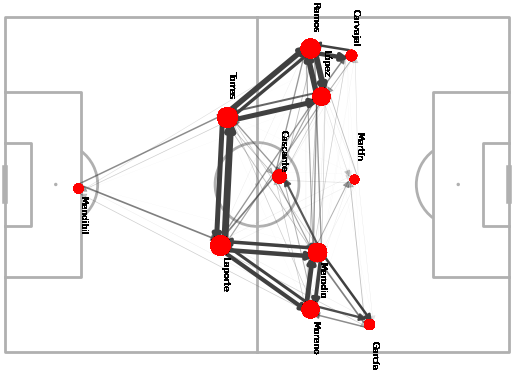
\includegraphics[width=0.7\textwidth]{../NoSubs/ImagesToRedo/Spain_Network_Spain_Sweden.png}
        \caption{Spain-Sweden}
        \label{fig: spain_sweden}
\end{figure}
As you can easily see this network is perfectly symmetric and this can make us recognize a pattern of play. This match is the most interesting example of the way the Spanish team plays, but starting from this, we can see that the Spanish team plays in a very similar way in almost all the matches. \\
\begin{figure}[H]
        \centering
        \subfloat[\centering Spain-Poland]{{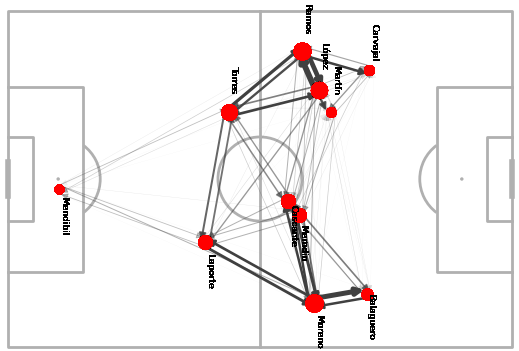
\includegraphics[width=0.4\textwidth]{../NoSubs/ImagesToRedo/Spain_Network_Spain_Poland.png} }}%
        \qquad
        \subfloat[\centering Switzerland-Spain]{{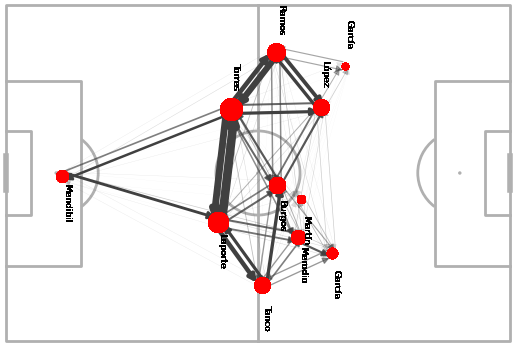
\includegraphics[width=0.4\textwidth]{../NoSubs/ImagesToRedo/Spain_Network_Switzerland_Spain.png} }}%
        \label{fig: spain_pattern}%
\end{figure}

Other interesting examples are the networks of Russia against Denmark (d) and Poland against Spain (c). In these two matches the strongest tie between two players is a pass from the goalkeeper to the centre forward. This is due to the difference of quality between the two teams and the high pressing the two opponent teams made during these matches, so the only playing possibility for Poland and Russia were to pass the ball back to the goalkeeper and he had the only choice to make a long pass toward the striker. \\


\begin{figure}[H]
        \centering
        \subfloat[\centering Poland in Spain-Poland]{{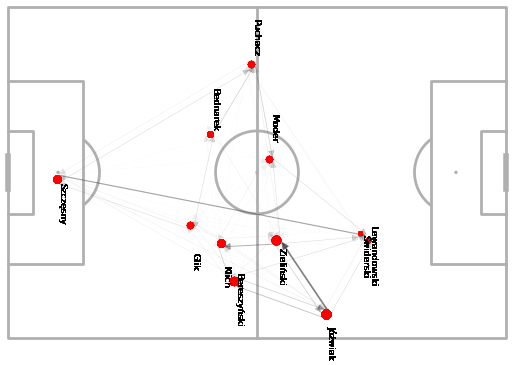
\includegraphics[width=0.4\textwidth]{../NoSubs/ImagesToRedo/Poland_Network_Spain_Poland.png} }}%
        \qquad
        \subfloat[\centering Russia in Russia-Denmark]{{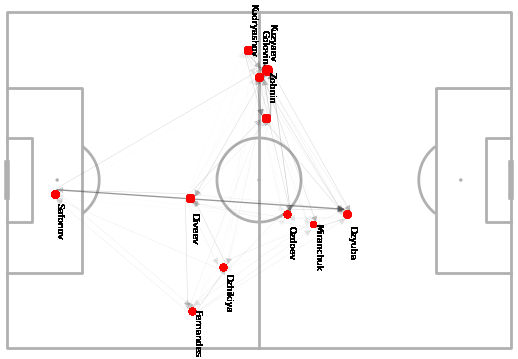
\includegraphics[width=0.4\textwidth]{../NoSubs/ImagesToRedo/Russia_Network_Russia_Denmark.png} }}%
        \label{fig:example}%
\end{figure}

\subsubsection{Node Centrality}
For each match and for each team we computed a weighted in-degree node centrality for each player. We used the in-degree centrality beacuse we are interested in how much other players in a team look for a certain player during a match. We then computed the average weighted centrality for each player, for each team. In some cases the results match our expectations, in others they do not. \\
The most evident example, in which the difference between the average weighted centrality and the weighted centrality of a player is very high, is the case of the Croatia team. Given that Luka Modric (Croatia's captain) is one of the most important players in the world, and moreover in the football history, we did expect him to be the most important node in Croatia's networks. This hypothesis is totally confirmed as Modric is the node with the highest centrality in three out of four matches played by Croatia in the tournament. The only match in which Modric is not the most important node in the network is the one against the Spain, in which Croatia has been eliminated from the tournament losing 3-5. The reason behind the fact that in this match Croatia's captain was not the most important node is related to the high pressing Spain midfielders have done on him in that match. This is a fantastic explanation of how analyzing the network structure of a team can be very useful to gain information about the style of play of opponent teams and to take countermeasures. \\ 

\begin{table}[H]
    \centering
    \begin{tabular}{|c|c|c|c|}
            \hline
            \textbf{Opponent} &  \textbf{Highest centrality} &  \textbf{Second highest centrality} &  \textbf{Mean} \\
            \hline
            \textbf{Czech Republic} &  Modric: $0.1645$ & Lovren: $0.1348$ & $0.0909$ \\
            \hline
            \textbf{ Scotland} &  Modric: $0.1621$ & Brozovic: $0.1439$ & $0.0909$ \\
            \hline
            \textbf{England} &  Modric: $0.1643$ & Kovacic: $0.1388$ & $0.0909$ \\
            \hline
            \textbf{Spain} &  Brozovic: $0.1745$ & Modric: $0.1236$ & $0.0909$ \\
            \hline
            \textbf{Total Sum} &  Modric: $0.6145$ & Kovacic: $0.4960$ & $0.3636$ \\
            \hline
    \end{tabular}
    \caption{Croatia's node in-degree centrality}
\end{table}

\begin{figure}[H]
    \centering
    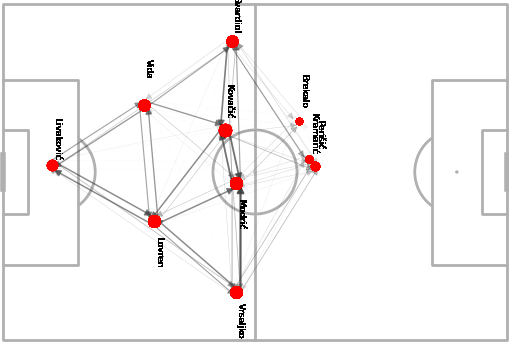
\includegraphics[width=0.7\textwidth]{../NoSubs/ImagesToRedo/Croatia_Network_Croatia_Czech Republic.png}
    \caption{Croatia-Czech Republic}
    \label{fig: spain_sweden}
\end{figure}


We expected to find the same result for Portugal, as Cristiano Ronaldo is the most important player in the team. However, this is not the case, as the average weighted centrality of Ronaldo is lower than the weighted centrality of the other players. This is due to the fact that Ronaldo as a striker is not involved in the build-up of the play. The top two players for node centrality have been Ruben Dias and Pepe, the two centre back. This is the case of the majority of the teams for example Spain, England, France, Sweden, Ukraine and so on. This is due to two main factors: the evolution of the style of play of football teams which prefers to keep the ball possession involving a lot the centre back in the build up and the fact that more and more teams are no longer using a striker who acts as a pivot and prefers a more mobile striker. \\
An honourable mention to the winner of the tournament: Italy. We did expect that Jorginho Frello would be the most important node in the Italian network, and despite he is the most central node in just 2 matches on 7, he has the highest average centrality, confirming our hypothesis. It is important to note that in the most matches the two most important nodes for Italy have always been Jorginho Frello or Marco Verratti, two midfielders. One important exceptions is the match against Spain (one of the most difficult matches in the tournament for Italy) in which the most important node has been Giorgio Chiellini, the centre back, for the same reason as Croatia-Spain match. \\

\begin{figure}[H]
    \centering
    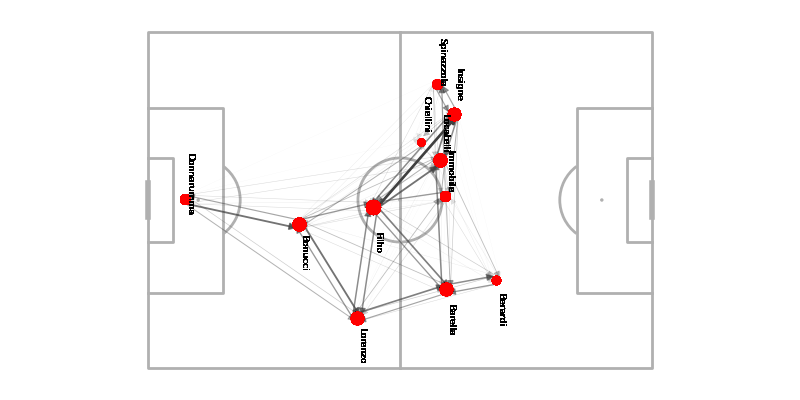
\includegraphics[width=0.7\textwidth]{../NoSubs/ImagesToRedo/Italy_Network_Italy_Switzerland.png}
    \caption{Italy-Switzerland}
    \label{fig: spain_sweden}
\end{figure}

%%%%%%%%%%%%%%%%%
%What is the connection among the gathered data, the applied measures,
%and the properties found?

\subsection{Conclusion}
\label{conclusion}
During a football match, the players of a team are constantly in contact with each other. The main way in which the players interact with each other is through passes. These passes create a network, representing the way the players of a team interact and so, the way the team plays.\\
In this study we analyzed 102 networks, from 24 different national teams in the Euro 2020 tournament. We have chosen Euro 2020 for three main reasons: the dataset was open, it is the last international tournament played and, being an international tournament with knockout games, the level of players and intensity of the matches is higher.\\
Using the network structure of a team we focused on two main aspects: the performance of a team and the style of play of a team, the first performed by a quantitative analysis of the network structure and the second by a qualitative analysis of the network structure.\\
This study has shown that the network structure of a team can be a very useful tool to understand the performance of a team. We started with two hypotheses to test:
\begin{itemize}
        \item Increasing the intensity of a network increase the team performance.
        \item Increasing the centralization of a network decrease the team performance. 
\end{itemize}
We have shown that data make us think that hypotheses are true, but we can't firmly assert that they are.\\
Another interesting perspective of this study is how the network structure of a team can be a useful tool to understand the team's style of play. We showed that observing the structure of a network is easy to recognize patterns of play, we showed the most evident one showing Spain's networks. After that we analyzed the in-degree centrality of nodes (players) in networks 
to understand which player is the most important in the network. We showed that the most evident case is the Croatia's one in which Modric is the most important node in all matches, except one: the match against Spain in which Spain's midfielders obstruct Croatia blocking Modric. This is the most important example we found on how analyzing a network can lead to new tactics that could be decisive in a tournament like this. \\
In conclusion this study has shown how important analyzing the structure of the network of a team could be in order to modify the style of play of a team and to counter the style of play of the opponent team. We tried to show how much these type of analysis can be useful to maximize the results of a team in the context of football, where the data analysis is still a growing field and a lot of teams do not apply this type of knowledge.\\

\subsubsection{Critique}
\label{critique}
In this study we would like to repeat the results obtained by another study \cite{GRUND} to test if the two hypothesis are true in a different context like an international tournament. The main difference between a domestic league and an international tournament is the level of players and the intensity of the matches. In a domestic league the level of the players is lower and the matches are less intense because  (especially during the first months of the competition) a single match is rarely decisive. This is confirmed by the fact that our data for network intensity are higher in comparison to the other study's data. 
We think that the main problem of our study is related to the limited quantity of data. Grund's study has analyzed two seasons of a domestic league (38 matches for 20 teams) for a total of 1520 networks while the Euro 2020 is a summer tournament played in a 3-4 weeks time span. Moreover, being Euro 2020 a knockout tournament half of the teams are eliminated after just three games, and only two teams play the full tournament (reaching the final) with a total of 7 matches. This is the main reason why we have a limited quantity of data if we want to perform this type of analysis on an international tournament. \\
As said earlier, due to Grund's methodology not being very clear, we have not been able to replicate his findings.\\
In conclusion, given the structure of football data, we couldn't apply other measures and analysis, like the study of cliques and cores in the network, as all players have a link with all others. This is the same reason for which we computed the network intensity instead of the network density. \\


%Do you think your work solves the problem presented above? To which
%extent (completely, what parts)? Why? What could you have done
%differently to answer your research problems (e.g., gather data with
%additional information, build your model differently, apply alternative
%measures)?

\bibliographystyle{plain}
\bibliography{bibliography}
\nocite{*}
\end{document}
